% Drawing 138/03-1 -- folder 138, batch 03, archive page 43 (PDF page 44).
% Transcription: à gauche, une sphère parcourue de trois grands cercles, les points d'intersection marqués $0$, $1$, $\infty$ (chacun deux fois) ; au-dessous, une seconde figure : une courbe fermée contenant un ovale, avec les points $\infty$, $0$, $1$, $0$, $\infty$ et deux traits marqués $1$.
% Kind: sphere with great circles; closed curve with oval. Method 2 (schematic redraw from the facsimile). Status: partial.
% Notes: Top: a sphere drawn as three closed curves, the « great circles »: the equator (an ellipse, with a small gap at its left end) through 0 (left, open point), 1 (upper right), 0 (right, open point), a dot, and 1 (lower left); a circle through infinity (top), the left 0, infinity (bottom) and the right 0; a circle through infinity (top), the upper 1, infinity (bottom) and the lower 1 (its lower end dips below the bottom infinity, as on the page). Every circle passes through the same intersection points. The axis through the two infinities: a stroke above the top one, a stroke below the bottom one, and between them, inside the sphere, the dashed line he drew (faint dashes). Below: a closed curve (bottom stroke wavy) with infinity at the top and at the bottom (on the curve), containing an oval through 0 (upper right) and 0 (lower left), crossed by a short stroke 1 at its left and at its right end, and a faint pencil arc inside the right part. Still differs: the circles are traced through points read on a 300 dpi crop, so their course is only as good as the reading (about one unit); his doubled stroke on the right side of the sphere (two pencil passes near the upper right) is drawn once; the left part of the circle through the 0s is broken at the label 0 as on the page. The « NB » paragraph and the 2 2 2 table at the bottom are text. Nothing is struck. Redrawn 2026-11-09 (issue 128): to check again.
% Coordinates: 1 unit = 1 mm = 1/100 of the crop width (bbox in page fractions: [0.1, 0.48, 0.32, 0.8]).
% Redrawn by Claude (claude-opus-5-5), issue #73, 2026-11-09; not checked by a human; not compiled (no TeX in the session).
% Rights: reproduces part of the work -- behind RENDER_TRANSCRIPTS, never published by itself.
\documentclass[tikz,border=3pt]{standalone}
\usepackage{amsmath,amssymb}
\usetikzlibrary{patterns,arrows.meta}
\tikzset{pencil/.style={black!45}, struck/.style={black!35}, mark/.style={circle,draw,inner sep=1.3pt}, pt/.style={circle,fill,inner sep=0.9pt}, opt/.style={circle,draw,fill=white,inner sep=1.1pt}}
\begin{document}
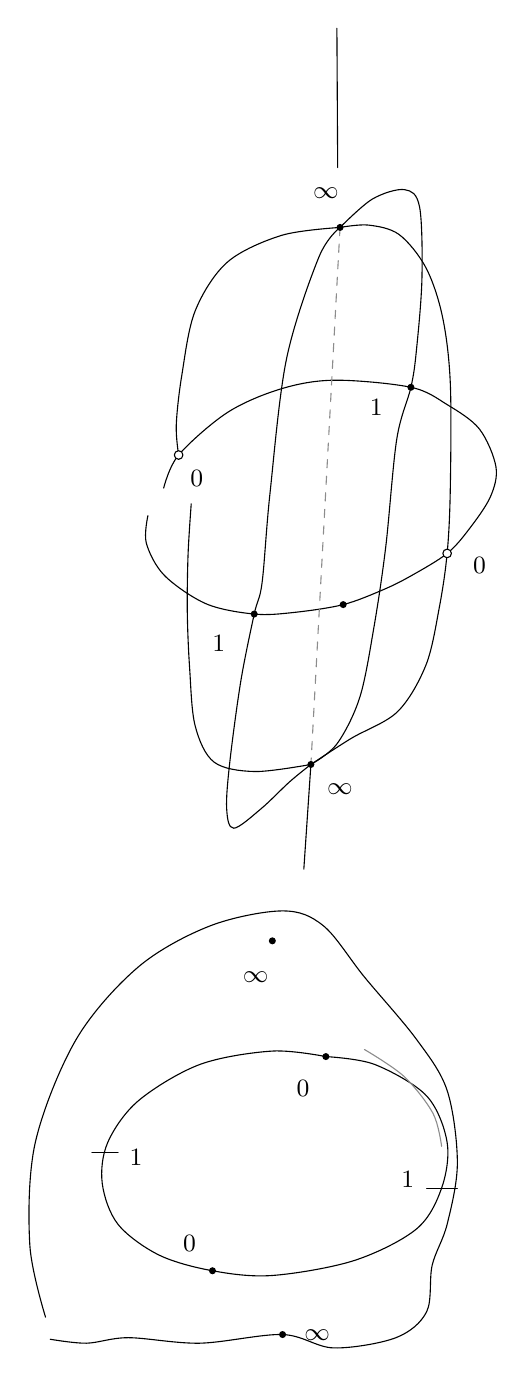
\begin{tikzpicture}[x=1mm,y=1mm,line cap=round,line join=round,font=\scriptsize]
\draw plot[smooth, tension=0.55] coordinates {(23.5,-60.7) (25.4,-56.5) (31.6,-51.1) (38.4,-48.1) (45.2,-47) (54.9,-47.9) (59.5,-50.1) (63.6,-53.2) (65.7,-58) (65,-61.8) (62.3,-65.9) (59.5,-69) (55,-71.8) (51.4,-73.6) (46.3,-75.5) (40,-76.5) (35,-76.7) (28.9,-75.4) (23.6,-71.8) (21.3,-67.7) (21.5,-64.2)};
\draw plot[smooth, tension=0.55] coordinates {(45.9,-27.6) (38.5,-28.6) (31.6,-32) (27.5,-38.2) (25.8,-46.4) (25.1,-52.7) (25.4,-56.5)};
\draw plot[smooth, tension=0.55] coordinates {(27,-62.7) (26.6,-69.1) (26.5,-76.4) (26.8,-83.6) (27.5,-90.9) (29.9,-95.5) (35.1,-96.7) (42.2,-95.8)};
\draw plot[smooth, tension=0.55] coordinates {(42.2,-95.8) (47.3,-92.5) (53.2,-89.1) (56.8,-83.2) (58.5,-75.9) (59.5,-69) (59.9,-60.9) (59.9,-47.3) (58.9,-38.9) (56.8,-32.7) (53.4,-28.5) (49.5,-27.3) (45.9,-27.6)};
\draw plot[smooth, tension=0.55] coordinates {(45.9,-27.6) (50,-24) (54.1,-22.8) (56,-25) (56.3,-34.1) (55.6,-43.2) (54.9,-47.9) (53.1,-54.5) (51.7,-68.2) (50.2,-78.4) (48.4,-87.3) (45.5,-93.2) (42.2,-95.8)};
\draw plot[smooth, tension=0.55] coordinates {(45.9,-27.6) (43.2,-31.4) (39.1,-44.3) (37,-61.4) (36,-72.7) (35,-76.7) (33.3,-85.2) (31.9,-95.5) (31.5,-101.4) (32.4,-103.9) (35.9,-101.4) (39.5,-98) (42.2,-95.8)};
\draw[dashed,pencil] (45.9,-27.6) -- (42.2,-95.8);
\draw (45.5,-2.3) -- (45.6,-20);
\draw (42.2,-95.8) -- (41.3,-109.1);
\node[pt] at (45.9,-27.6) {};
\node[pt] at (54.9,-47.9) {};
\node[pt] at (35,-76.7) {};
\node[pt] at (42.2,-95.8) {};
\node[pt] at (46.3,-75.5) {};
\node[opt] at (25.4,-56.5) {};
\node[opt] at (59.5,-69) {};
\node[inner sep=1pt] at (44.1,-23.2) {\small $\infty$};
\node[inner sep=1pt] at (27.7,-59.5) {\small $0$};
\node[inner sep=1pt] at (50.5,-50.5) {\small $1$};
\node[inner sep=1pt] at (63.6,-70.5) {\small $0$};
\node[inner sep=1pt] at (30.5,-80.5) {\small $1$};
\node[inner sep=1pt] at (45.9,-98.9) {\small $\infty$};
\draw plot[smooth, tension=0.55] coordinates {(8.5,-166) (6.5,-156.8) (7.2,-143.8) (12.4,-130.7) (20.3,-121.5) (29.4,-116.3) (38.6,-114.4) (43.8,-116.3) (49,-122.8) (55.6,-130.7) (59.5,-137.2) (60.8,-146.4) (59.5,-154.2) (57.6,-159.4) (56.9,-165.3) (53,-168.6) (45.1,-169.9) (38.6,-168.2) (28.1,-169.3) (19,-168.6) (13.7,-169.3) (9.1,-168.8)};
\draw plot[smooth, tension=0.55] coordinates {(44.1,-132.9) (37.3,-132.2) (28.1,-133.9) (20.3,-138.5) (16.4,-143.8) (15.7,-149) (17.7,-154.2) (22.9,-158.1) (29.7,-160.1) (37.3,-160.7) (47.7,-158.8) (55.6,-154.8) (58.8,-149.6) (59.5,-143.8) (56.9,-137.9) (50.3,-133.9) (44.1,-132.9)};
\draw[pencil] plot[smooth, tension=0.55] coordinates {(49,-132) (54,-135.4) (57.7,-140.1) (58.8,-144.3)};
\draw (14.4,-145.1) -- (17.7,-145.1);
\draw (56.9,-149.6) -- (60.8,-149.6);
\node[pt] at (37.3,-118.2) {};
\node[pt] at (44.1,-132.9) {};
\node[pt] at (29.7,-160.1) {};
\node[pt] at (38.6,-168.2) {};
\node[inner sep=1pt] at (35.2,-122.8) {\small $\infty$};
\node[inner sep=1pt] at (41.2,-137) {\small $0$};
\node[inner sep=1pt] at (26.8,-156.6) {\small $0$};
\node[inner sep=1pt] at (20,-145.7) {\small $1$};
\node[inner sep=1pt] at (54.5,-148.5) {\small $1$};
\node[inner sep=1pt] at (43,-168.3) {\small $\infty$};
\end{tikzpicture}
\end{document}
